% %%%%%%%%%%%%%%%%%%%%%%%%%%%%%%%%%%%%%%%%%%%%%%%%%%%%%%%%%%%%%%%%%%%%%%%%%%%%%%%
\documentclass[letterpaper, 10 pt, conference]{ieeeconf}  % Comment this line out if you need a4paper

%\documentclass[a4paper, 10pt, conference]{ieeeconf}      % Use this line for a4 paper

\IEEEoverridecommandlockouts                              % This command is only needed if 
% you want to use the \thanks command

\overrideIEEEmargins                                      % Needed to meet printer requirements.




%\documentclass[journal,letterpaper]{IEEEtran}
% include the list of acronyms, math commands and new commands used in this paper
% \usepackage[backend=bibtex,maxnames=2]{biblatex}
\usepackage[pdftex]{graphicx}
%\usepackage[numbers]{natbib}
\bibliographystyle{IEEEtran}
\usepackage{booktabs}
\usepackage{moreverb}
%\usepackage{titlesec}
%\usepackage[titletoc,toc,title]{appendix}
\usepackage{url}
\usepackage{amsmath}
\usepackage{multicol,lipsum}
\usepackage{mathtools}
\usepackage{cuted}
\usepackage{amsfonts}
\usepackage{multirow}
\usepackage{bm}
\usepackage{subfig}
\usepackage{color, colortbl}
\usepackage[colorlinks,bookmarksopen,bookmarksnumbered,citecolor=red,urlcolor=red]{hyperref}

%\usepackage{enumitem}

\hypersetup
{
	pdftitle = {Whole-body control for quadrupedal locomotion on challenging terrain},
	pdfauthor = {Francesco Roscia},
	pdfsubject = {RA-L manuscript},
	pdfkeywords = {legged robots, aerial locomotion, and safe landing},
	pdftoolbar = true,
	colorlinks = true,
	linkcolor = black,
	citecolor = black,
	urlcolor = black,
}

\usepackage[usenames,dvipsnames]{xcolor}%\usepackage{xcolor,colortbl}
\definecolor{blue_iit}{RGB}{51,51,255}
\usepackage{algpseudocode}
\usepackage{algorithm}


\usepackage[acronym,hyperfirst=false]{glossaries}

\usepackage[tight]{units}
\usepackage[normalem]{ulem} % to strike out text, use: \sout{text}
\usepackage{cancel}
\definecolor{Gray}{gray}{0.9}
\usepackage{tensor} 
\usepackage{nicefrac}
%\usepackage{cleveref}
%\crefname{figure}{Fig.}{Fig.}
%\crefname{equation}{Eq.}{Eq.}
%\AtBeginDocument{%
%  \renewcommand{\crefpairconjunction}{,}%% instead of " and\nobreakspace"
%  \renewcommand{\crefmiddleconjunction}{,}% instead of ", "
%  \renewcommand{\creflastconjunction}{,}% instead of " and\nobreakspace"
%}
\usepackage[sorting=none, style=ieee]{biblatex}
\addbibresource{references/bibliography.bib} 
\newacronym{hyq}{HyQ}{Hydraulically actuated Quadruped}

\newacronym{lf}{LF}{Left-Front}
\newacronym{rf}{RF}{Right-Front}
\newacronym{lh}{LH}{Left-Hind}
\newacronym{rh}{RH}{Right-Hind}

\newacronym{haa}{HAA}{Hip Adduction-Abduction}
\newacronym{hfe}{HFE}{Hip Flexion-Extension}
\newacronym{kfe}{KFE}{Knee Flexion-Extension}

\newacronym{imu}{IMU}{Inertial Measurement Unit}
\newacronym{dofs}{DoFs}{Degrees of Freedom}
\newacronym{rt}{RT}{Real Time}

\newacronym{com}{CoM}{Center of Mass}
\newacronym{cop}{CoP}{Center of Pressure}
\newacronym{zmp}{ZMP}{Zero Moment Point}
\newacronym{icp}{ICP}{Instantaneous Capture Point}
\newacronym{cp}{CP}{Capture Point}
\newacronym{cmp}{CMP}{Centroidal Moment Pivot}
\newacronym{grfs}{GRFs}{Ground Reaction Forces}

\newacronym{ls}{LS}{Least Square}

\newacronym{slip}{SLIP}{Spring Loaded Inverted Pendulum}
\newacronym{eom}{EoM}{Equation of Motions}
\newacronym{qp}{QP}{Quadratic Program}
\newacronym{sqp}{SQP}{Sequential Quadratic Programming}
\newacronym{mic}{MIC}{Mixed-Integer Convex}
\newacronym{cmaes}{CMA-ES}{Covariance Matrix Adaptation Evolution Strategy}
\newacronym{ara}{ARA*}{Anytime Repairing A*}
\newacronym{pca}{PCA}{Principal Component Analysis}
\newacronym{cpg}{CPG}{Central Pattern Generator}
\newacronym{wbc}{WBC}{Whole-Body Control}

\newacronym{mpc}{MPC}{Model Predictive Control}
\newacronym{ik}{IK}{Inverse Kinematic}
\newacronym{ocp}{OCP}{Optimal Control Problem}
\newacronym{nlp}{NLP}{Nonlinear Programming}
\newacronym{ltv}{LTV}{Linear Time Varying}


% SOFT TERRAIN ADAPTATION
\newacronym{awbc}{c$^3$WBC}{Compliant Contact Consistent Whole-Body Control}
\newacronym{swbc}{sWBC}{Standard Whole-Body Control}
\newacronym{c3wbc}{c$^3$WBC}{Compliant Contact Consistent Whole-Body Control}
\newacronym{ste}{TCE}{Terrain Compliance Estimator}
\newacronym{c3}{\texttt{c}$^3$}{compliant contact consistent}

\newacronym{stance}{STANCE}{\textbf{S}oft \textbf{T}errain \textbf{A}daptation a\textbf{n}d \textbf{C}ompliance \textbf{E}stimation}

\newacronym{wbopt}{WBOpt}{Whole Body Optimization}


\newacronym{hc}{HC}{Hunt and Crossley's}
\newacronym{kv}{KV}{Kelvin-Voigt's}

\newacronym{wllsr}{WLLSR}{Weighted Linear Least Squared Regression}

\newcommand{\grfs}{\gls{grfs}~}

\newacronym{mae}{MAE}{Mean Absolute Tracking Error}

\newacronym{ode}{ODE}{Open Dynamics Engine}

\newacronym{cmg}{CMG}{Control Moment Gyroscope}
\newacronym{ocs}{OCS}{Orientation Control System}
\newcommand{\reducespace}{\vspace{-1.5em}}
%\newcommand{\reducespace}{\vspace{0em}}
\newcommand{\Rnum}{\mathbb{R}} % Symbol fo the real numbers set
\newcommand{\hf}{\textsc{hf}}
\newcommand{\vect}[1]{\mathbf{#1}} %vector bold

\newcommand{\grf}{F_{\mathrm{grf}}} % vector to denote the contact forces, ground reaction forces
\newcommand{\grfp}[1]{F_{\mathrm{grf,#1}}} % vector to denote the contact forces, ground reaction forces
\newcommand{\grfest}[1]{F_{\mathrm{grf},#1}} % vector to denote the contact forces, ground reaction forces

\newcommand{\mrm}[1]{\mathrm{#1}}
\newcommand{\nmrm}[1]{{#1}}
\newcommand{\fratop}[2]{\genfrac{}{}{0pt}{}{#1}{#2}}
\newcommand{\mx}[1]{\mathbf{\bm{#1}}} 				% Matrix symbol
%\newcommand{\vc}[1]{\mathbf{\bm{#1}}} 					% Vector symbol
\newcommand{\vc}[1]{#1}
\newcommand{\degree}{\ensuremath{^\circ}}				% define the degree symbol
\newcommand{\pder}[2]{\frac{\partial#1}{\partial#2}}		% partial derivative
\newcommand{\refframe}[1]{\mbox{\textless#1\textgreater}}	% to denote a reference frame
\DeclareMathOperator*{\argmin}{\arg\!\min}				% argmin
\DeclareMathOperator*{\argmax}{\arg\!\max}				% argmax
\DeclareMathOperator*{\st}{s.t.}						% subject to
\DeclareMathOperator*{\dif}{\mathrm{d}}					% d
\DeclareMathOperator*{\half}{\frac{1}{2}}					% one half
\newcommand{\mat}[1]{\ensuremath{\begin{bmatrix}#1\end{bmatrix}}}	% matrix
\newcommand{\rank}[1]{\text{rank}(#1)}							% rank
\newcommand{\diag}[1]{\text{diag}(#1)}							% diag
\newcommand{\x}{\ensuremath{\times}}
\newcommand{\dx}[1]{\ensuremath{\delta x_{#1}}}					% dx
\newcommand{\du}[1]{\ensuremath{\delta u_{#1}}}					% du
\newcommand{\DX}[0]{\ensuremath{\Delta X}}						% DX
\newcommand{\DU}[0]{\ensuremath{\Delta U}}						% DU
\newcommand{\ith}[0]{\ensuremath{i^\text{th}}}					% i-th
\newcommand{\T}[0]{\ensuremath{\top}}							% transpose symbol
%\newcommand{\Rv}[1]{\ensuremath{\mathbb{R}^{#1}}}				% set of real-valued vectors
%\newcommand{\R}[2]{\ensuremath{\mathbb{R}^{#1\times #2}}}		% set of real-valued matrices
\newcommand{\Spd}[1]{\ensuremath{\mathbb{S}_+^{#1}}}			% set of symmetric positive-definite matrices
\newcommand*\rfrac[2]{{}^{#1}\!/_{#2}}%running fraction with slash - requires
% math mode.

\newcommand{\crossmx}[1]{\mat{#1}_{\times}} %vector bold

\newcommand\bovermat[2]{\makebox[0pt][l]{$\smash{\overbrace{\phantom{%
    \begin{matrix}#2\end{matrix}}}^{\text{#1}}}$}#2}

\newcommand{\annotation}[1]{\footnote{\color{red}{#1} }}
\usepackage{mathtools}
\DeclarePairedDelimiter{\abs}{\lvert}{\rvert}
\DeclarePairedDelimiterX{\norm}[1]{\lVert}{\rVert}{#1}
\newcommand{\sref}[1]{Section~\ref{#1}}
%\newcommand{\eref}[1]{Eq.~(\ref{#1})}
\newcommand{\eref}[1]{(\ref{#1})}
\newcommand{\fref}[1]{Fig.~\ref{#1}}
\newcommand{\tref}[1]{Table~\ref{#1}}



%\newtheorem{Assumption}{Assumption}[section]
\newtheorem{assump}{Assumption}
\newtheorem{assumpB}{Assumption}
\renewcommand\theassump{1}
\renewcommand\theassumpB{2}
\newcommand{\assref}[1]{Assumption~\ref{#1}}


\newcommand{\MF}[1]{\textcolor{red}{\textbf{mfocchi}: #1}}
\newcommand{\CS}[1]{\textcolor{violet}{\textbf{csemini}: #1}}
\newcommand{\FR}[1]{\textcolor{teal}{\textbf{froscia}: #1}}



\newcommand\BibTeX{{\rmfamily B\kern-.05em \textsc{i\kern-.025em b}\kern-.08em
T\kern-.1667em\lower.7ex\hbox{E}\kern-.125emX}}


\newcommand{\ie}{{i.e.},\ }
\newcommand{\eg}{{e.g.},\ }
\newcommand{\etal}{{\textit{et~al.}}\ }


\captionsetup[table]{labelsep=newline}
\captionsetup[table]{justification=centering}



\makeatletter
\newcounter{definition*}
\newenvironment{definition*}[1][htb]
{\renewcommand{\ALG@name}{Definition}% Update algorithm name
	\let\c@algocf\c@megaalgorithm% Update algorithm counter
	\begin{algorithm*}[#1]%
	}{\end{algorithm*}}
\makeatother

\makeatletter
\newcounter{definition}
\newenvironment{definition}[1][t]
{\renewcommand{\ALG@name}{Proposition}% Update algorithm name
	\let\c@algocf\c@megaalgorithm% Update algorithm counter
	\begin{algorithm}[#1]%
	}{\end{algorithm}}
\makeatother

\newcommand{\defref}[1]{Proposition~\ref{#1}}


%\usepackage[table]{xcolor}
\definecolor{sfahmi_blue}{RGB}{0.19,0.51,0.74}
%\definecolor{DarkGray}{RGB}{0.25,0.25,0.25}
%\definecolor{Gray}{RGB}{0.5,0.5,0.5}
%\definecolor{Red}{RGB}{1,0,0}
\definecolor{LightBlue}{RGB}{0.4,0.4,1}
\newcommand{\thickhline}{\noalign{\hrule height 0.8pt}}

\newcommand{\bmcolor}[1]{\textcolor{RoyalBlue}{\bm{#1}}}


\hypersetup{draft}
\makeglossaries

\title{Orientation Control System: Enhancing Aerial Maneuvers \\ for Quadruped Robots}
\author{
	Francesco Roscia$^{1}$, Andrea Cumerlotti$^{1, \, 2}$, Andrea Del Prete$^{2}$, Claudio Semini$^{1}$, and Michele Focchi$^{1, \, 3}$
	\thanks{$^1$ Dynamic Legged Systems (DLS) lab, Istituto Italiano di Tecnologia (IIT), Genoa, Italy.
		$^2$ Industrial Engineering Department (DII), University of Trento, Trento, Italy.
		$^3$ Department of Information Engineering and Computer Science (DISI), University of Trento, Trento, Italy.
}}


\begin{document}
\maketitle
\thispagestyle{empty}
\pagestyle{empty}

\begin{abstract}%150-250 word abstract
For legged robots, aerial motions are the only option to overpass obstacles that cannot be circumvent with standard locomotion gaits. In these cases, the robot must perform a leap to either jump onto the obstacle or fly over it. However, these movements represent a challenge because during the flight phase the \gls{com} cannot be controlled, and the robot orientation has limited controllability. This paper focuses on the latter issue and proposes an \gls{ocs} consisting of two rotating and actuated masses (flywheels or reaction wheels) to gain control authority on the robot orientation. Because of the conservation of angular momentum, their rotational velocity can be adjusted to steer the robot orientation even when there are no contacts with the ground. The axes of rotation of the flywheels are designed to be incident, leading to a compact orientation control system that is capable of controlling both roll and pitch angles, considering the different moment of inertia in the two directions. We tested the concept with simulations on the robot Solo12.
\end{abstract}

%\begin{IEEEkeywords}
	 
%\end{IEEEkeywords}

\section{Introduction}\label{sec:introduction}
Legged robots are designed for traversing rough terrain.
Different types of gaits, such as trot or crawl, have been developed for quadrupedal robots. 
Thanks to the progress of the last two decades, robots have become lighter and stronger, which has enabled them to perform agile locomotion.
However, sometimes it is not possible to get around or over an obstacle with the gaits mentioned above, and jumps are required. 

When the robot is in the air, the \gls{com} moves on the ballistic trajectory, that is completely defined by the lift-off position and velocity. On the other hand, the base orientation can be changed exploiting the conservation of the system angular momentum. This means that it is possible to control the base angular velocity by changing the inertia of the robot, e.g., changing the joints configuration. 

Nevertheless, the majority of quadrupeds are designed with light legs, resulting in limbs that have small influence on the total angular momentum.

\begin{figure}[t!]
	\centering
	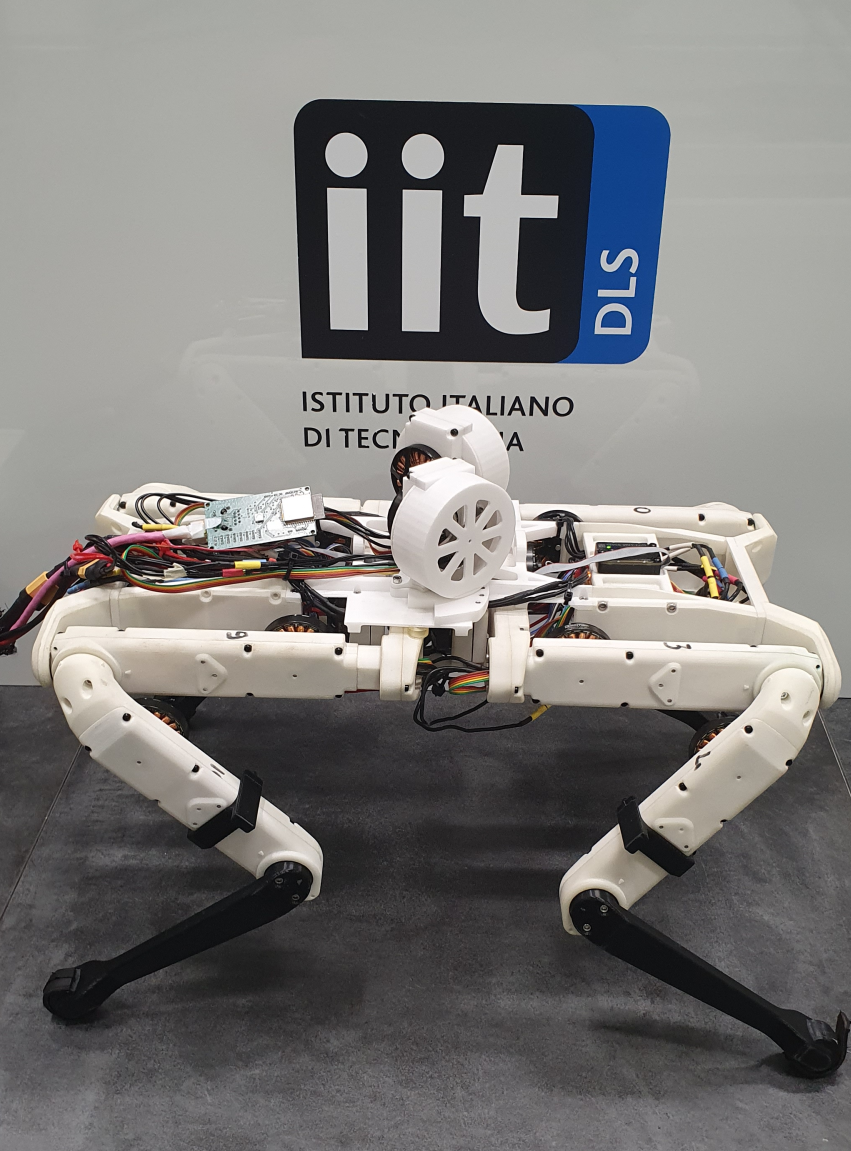
\includegraphics[width=.7\linewidth]{figures/solo_fw_pic_compressed.png}
	\caption{\small The proposed Orientation Control System for 
		for the $2.5 \ \mathrm{kg}$ quadruped robot Solo12 consists of two $0.1 \ \mathrm{kg}$ flywheels with incident rotation axes. Each wheel is located in a 3D-printed shell and mounted on the trunk body.}
	\label{fig:solo12flywheels}
\end{figure} 

Quadrupedal animals, like cats, can rearrange the tail and trunk to correct the orientation during a fall \cite{kane1969dynamical}.
% Tail
Many works in the field of robotics used an additional link as a tail, like in \cite{chu2019null} and \cite{wenger2016frontal}.
This link rotates around an axis that does not pass through the robot \gls{com}: the distances between the axis of rotation and the \gls{com} of both trunk and tail result in a large effect on the total angular momentum even with a small tail mass.
However, the placement of the additional link makes the resulting robot asymmetric. Moreover, due to its limited range of motion, a tail can be used only for a single jump, not for a repeated sequence~\cite{johnson2012tail}.
% Legs reconfig
It is possible to obtain a similar result by creating repetitive circular motions with the feet, like in \cite{hoffman2021exploiting} and \cite{kurtz2021mini}. In the latter work, the authors proposed special heavy boots for Mini Cheetah and used a neural network to calculate online joint trajectories. However, this solution unnecessarily increases the inertia of the legs, complicating the locomotion problem, which can no longer rely on the massless leg assumption. %\annotation{trova un modo per dire che questa complicazione è data dalla massless assumption che non è più valida} 
% Gyros
Another option is to use a \gls{cmg}.
It consists of a wheel, spinning at a constant angular velocity inside two or three actuated gimbals.
Tilting the wheel's axis of rotation generates the gyroscopic torque.
This system is widespread in spacecrafts reorientation \cite{yoon2002spacecraft}, but less frequently exploited in robot locomotion, either wheeled \cite{brown1996single} or legged \cite{mikhalkov2021gyrubot}.
The \gls{cmg} presents interesting capabilities, but the presence of a pan-tilt unit to drive the gyroscope makes it impractical to mount it on a small, lightweight robot.

% flywheel
flywheels represent an additional option for controlling the robot orientation.
Changing the angular velocity of a rotating mass attached to the trunk generates a torque that can reorient the robot. This device has been first applied for spacecraft orientation \cite{oland2009reaction}, and later it has been only sporadically investigated in legged locomotion for controlling pitch orientation, both for bipeds \cite{Brown2016}, \cite{xiong2020sequential} and quadrupeds \cite{kolvenbach2019towards}, \cite{vasilopoulos2016quadruped}.
Compared with tails, flywheels do not have position limits, and since their rotation axes pass through the \gls{com}, its angular momentum results holonomic \cite{machairas2015quadruped}.
To get a fast response, it is necessary to have an abrupt change in the flywheels angular velocity (angular acceleration).
Using a brake avoids the employment of a motor able to deliver higher torques \cite{gajamohan2012cubli}, 
keeping the system compact: the motor slowly accelerates the wheel to a certain speed to store angular momentum and, when a reorientation is required, the break stops its spin.
Since the effect of the break is unidirectional, a limitation of this approach is given by the fact that it is possible to generate a rotation of the base only in the opposite direction of the flywheel angular velocity making them unsuitable for applications where \textit{continuous} controllability is required. On the other hand, direct-drive controlled flywheels enable to create accelerations in both directions,  and  to implement continuous control laws. The benefits of this kind of  \gls{ocs} are multiple: 1) flywheels can correct orientation errors during the flight (e.g. due to disturbances or tracking inaccuracies in the angular momentum achieved at the lift-off)   % and non-idealities).  
in a continuous manner. 2) They enable to track a time-varying reference (e.g. to have the robot land with a desired angular velocity (possibly zero) and orientation).
3) Even in presence of contacts, they can enhance the landing phase or stabilize dynamic gaits (e.g. trot), by significantly reducing trunk oscillations.  
4) The presence of these additional joints, whose only function is to control the orientation, gives the possibility to relieve the effort of the legs.
In more complex scenarios, like for a somersault, limbs and \gls{ocs} can operate in parallel to achieve a rotation angle larger than the one achievable only with legs (e.g., due to torque limitation). 

\subsection{Proposed Approach and Contribution}
In this work, we present a compact \gls{ocs} based on two flywheels, mounted on the trunk of the lightweight quadruped Solo12 \cite{grimminger2020open}, see Fig. \ref{fig:solo12flywheels}. 
The contributions of the paper are:
\begin{itemize}
	\item the design of a novel \gls{ocs} that enables to control the orientation of a legged robot during a jump in an effective way, while keeping the design simple. 
	In particular,  the axes of rotation of the flywheels are set to be incident, enabling \textit{continuous} controllability in both the directions (roll and pitch) while keeping the  device compact.
	\item simulations  with the quadruped Solo12 that demonstrate the effectiveness of the proposed approach.
\end{itemize}



\subsection{Outline}
The reminder of this paper is organized as follow. In Section \ref{sec:background}, the law of conservation of the total angular momentum is recalled. In Section \ref{sec:ocs}, the design principles are presented together with the strategy for simultaneously control the robot roll and pitch orientations. Section \ref{sec:simulations} presents simulation in different scenarios that demonstrate the the capability of our \gls{ocs} to reject disturbances and to track angular references when there is no contact with the ground, and damping of base oscillation after the touch-down. Conclusions and a possible evolution of the work ar reported in Section \ref{sec:conclusions}.
% 

\section{Background}
\label{sec:background}
The starting point for any \gls{ocs} is the Euler's equation. For any mechanical system, the time derivative of the angular momentum $\bm{L}$ computed with the respect to a reference point $O$, fixed in an inertial frame, equals the sum of the moments $\bm{M}_i$ applied to the system with respect to the same reference point:
\begin{equation}
\dot{\bm{L}} = \sum_i \bm{M}_i
\end{equation}
When the resultant of the external moments applied to the system is zero, the Euler's equation simplifies to:
\begin{equation}
\dot{\bm{L}} = 0 \quad \Rightarrow \quad \bm{L}(t) = const,
\label{eq:cons_ang_mom}
\end{equation}
which is known as conservation of angular momentum.
Referring to legged robots, this condition occurs when the system is not in contact with the ground or other objects, e.g., during a fall or the flight phase of a jump.
In this case, it is possible to change the angular velocity of the base link changing the joint positions and velocities, as a result of the \textit{non-holonomy} of the total angular momentum \cite{Wieber16}: if the angular momentum of a certain body changes, the one of the others must change to maintain the total sum constant.

\section{Orientation Control System}
\label{sec:ocs}
In this section, we present a procedure to select the inertia of the flywheels, and we show how to exploit them for simultaneously controlling the robot roll and pitch orientation.
\subsection{Inertia Selection}
A preliminary analysis for the selection of the flywheels' inertia can be performed with the Elroy's Beanie model, depicted in Fig. \ref{fig:elroy-beanie}.
\begin{figure}
	\centering
	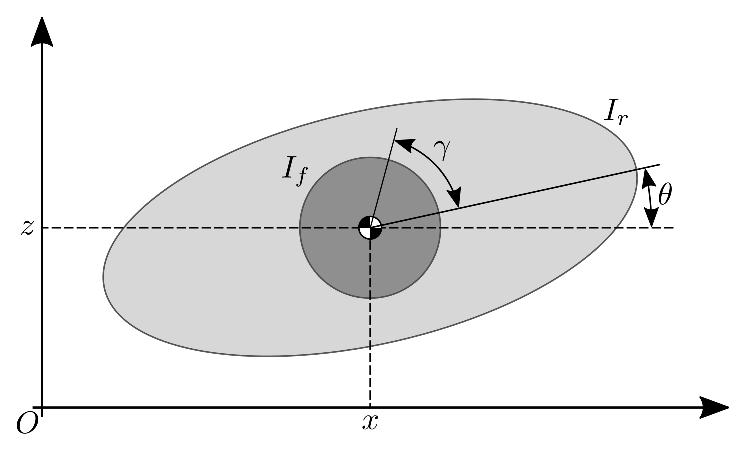
\includegraphics[width=.7\linewidth]{figures/elroys-beanie.eps}
	\caption{\small Schematic representation of the Elroy's Beanie model used for the preliminary analysis of the pitch motion.}
	\label{fig:elroy-beanie}
\end{figure} 
This consists of two rigid bodies connected through their \gls{com} with a revolute joint. One of the bodies represents the robot in its nominal configuration. The other models the \gls{ocs}, here represented by a single wheel for the sake of simplicity. The aim is to examine the rotational dynamics of the system as a whole. To simplify the analysis, in the following we will refer only to the effects on the pitch angle of the robot, keeping in mind that the same arguments apply also to the roll. 
Let us identify the moment of inertia of the robot in the nominal configuration as $I_r$ and the moment of inertia of the two flywheels as $I_f$, both referred to the system \gls{com}.
The angular momentum $L$ of this system can be written as
\begin{equation}\label{eq:ang_mom_elroy}
L(t) = \left(I_r + I_{f}\right)\dot{\theta}(t) + I_{f}\dot{\gamma}(t)
\end{equation}
where $\dot{\theta}$ and $\dot{\gamma}$ are respectively the robot pitch rate and the angular speed of the wheel.
We want to drive the robot to a desired pitch rate $\dot{\theta}_{des}$ by acting on the wheel speed.
Without loss of generality, we can assume the flywheel is stationary with the robot at the instant at which the reorientation maneuver starts ($\dot{\gamma}_0 = 0$), having a system angular momentum of $L_0 = \left(I_r + I_{f}\right)\dot{\theta}_0$.
Under the condition of conservation of the angular momentum, this quantity is constant over time and it is possible to estimate the lower bound for $I_{f}$ given a desired pitch rate and the maximum velocity of the flywheels $\dot{\gamma}_{max}$:
\begin{equation}
I_{f} \geq I_r \dfrac{ \Delta \dot{\theta} }{\Delta \dot{\theta}+\dot{\gamma}_{max}}.
\end{equation}
where $\Delta \dot{\theta} =  \left\lvert \dot{\theta}_0-\dot{\theta}_{des} \right\rvert$ is the base velocity variation.
Fig. \ref{fig:inertia_limits} reports the lower bound of $I_{f}$ given the desired base velocity variation and the maximum velocity of the actuator.
\begin{figure}
	\centering
	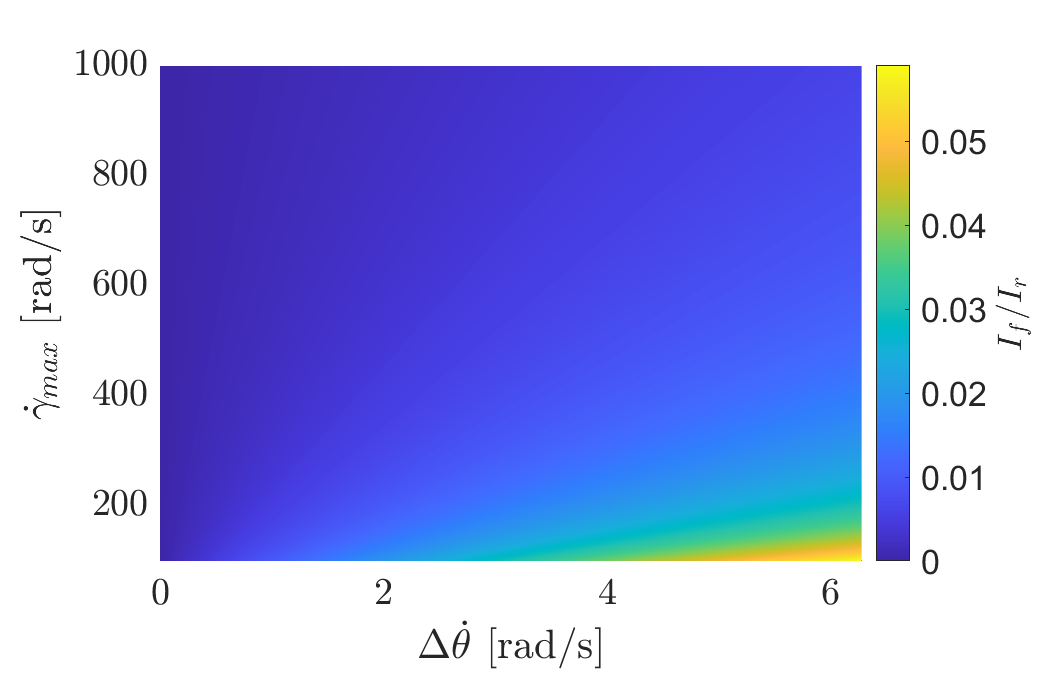
\includegraphics[width=\linewidth]{figures/lowerbound.eps}
	\caption{\small Minimum inertia of the \gls{ocs} (normalized by the robot inertia) necessary to achieve a base velocity variation $\Delta \dot{\theta}$, given the actuation bound $\dot \gamma^{max}$.}
	\label{fig:inertia_limits}
\end{figure}


\subsection{Flywheels Axes of Rotation}

The orientation of the axis of rotation of each flywheel influences their contribution to the total angular momentum. To meet the specification of controlling both the robot roll and pitch, the axes of rotation of the left and right wheel, identified in the base reference frame with the unit vectors $\hat{\bm{a}}_l$ and $\hat{\bm{a}}_r$, are set to be incident, laying on a plane parallel to the $xy-$plane of the base reference frame (see Fig. \ref{fig:axes}). 
To remove unnecessary complications, we designed two identical modules, to be mounted on the trunk of Solo12, symmetrically with the respect of the robot sagittal plane. We denote with $\alpha \leq \pi/2$ the non-negative incident angle between the wheels' axes of rotation and the robot lateral direction. The matrix 
\begin{equation}
\bm{C} = 
\left[ \begin{array}{cc}
\hat{\bm{a}}_l & \hat{\bm{a}}_r
\end{array} \right] = 
\left[ \begin{array}{cc}
\sin(\alpha) & -\sin(\alpha) \\
\cos(\alpha) & \cos(\alpha) \\
0 & 0
\end{array} \right]
\end{equation}
maps the flywheel moments into scalar torques $\bm{u} = \left[\begin{array}{cc} \tau_{fl} & \tau_{fr} \end{array} \right]^T$ about the flywheel axes $\hat{\bm{a}}_l$ and $\hat{\bm{a}}_r$ (expressed in the base frame).
As long as $\bm{C}$ is full column rank, it is possible to control both roll and pitch angles. If $\alpha = 0$, the roll results to be uncontrollable through the \gls{ocs}; otherwise, if $\alpha = \pi/2$, the pitch is uncontrollable. 
\begin{figure}
	\centering
	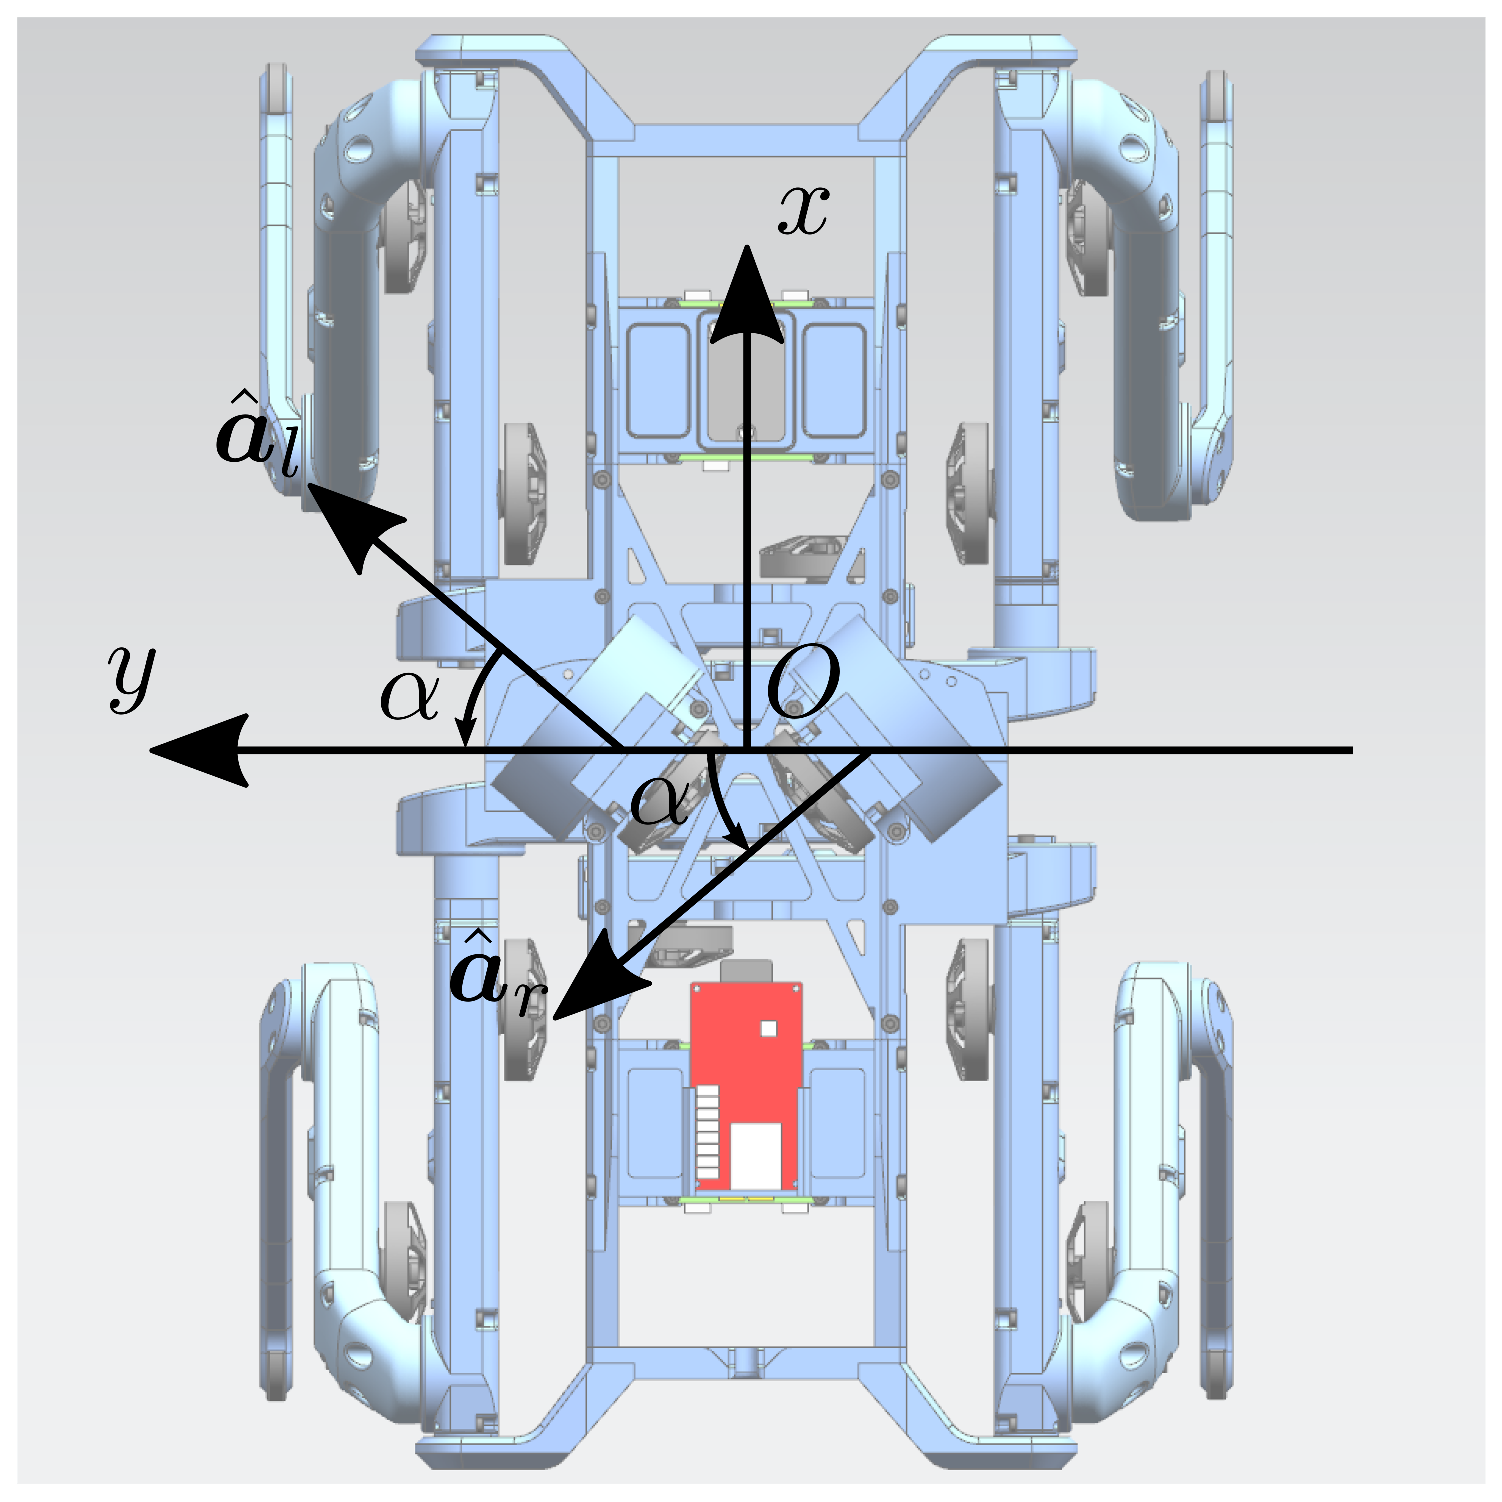
\includegraphics[width=0.7\linewidth]{figures/axes.eps}
	\caption{\small Representation of the flywheels rotation axes, seen from the top of the robot.}
	\label{fig:axes}
\end{figure}
The angle is selected considering the ratio of the eigenvalues along the $x$ and $y$ directions of the ellipsoid of the robot inertia(Fig. \ref{fig:ellipsoid}):
\begin{equation*}
\alpha^{*}=\tan^{-1}\left(\dfrac{I_{r, xx}}{I_{r, yy}}\right).
\end{equation*}
\begin{figure}
	\centering
	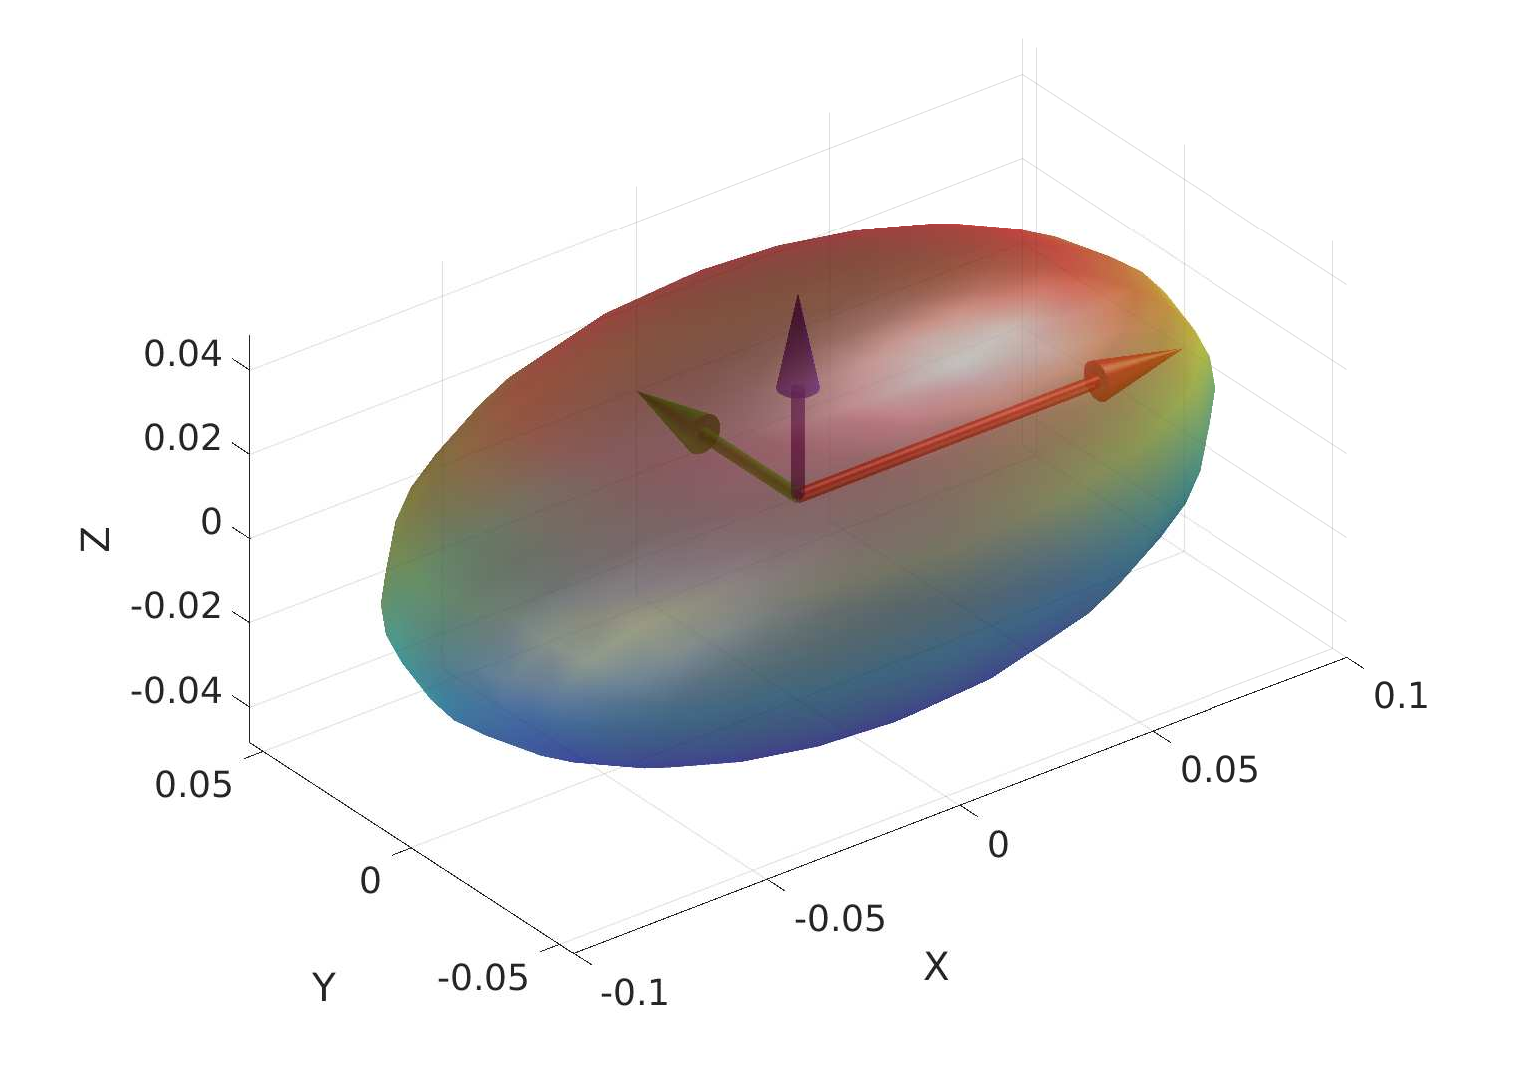
\includegraphics[width=1\linewidth]{figures/inertiaEllipsoid.eps}
	\caption{\small The inertia tensor can be seen as an ellipsoid. Its principal axes in the direction of the eigenvectors of the tensor and their length depends on the eigenvalues.}
	\label{fig:ellipsoid}
\end{figure}
In the case of Solo12, this angle is about $40^{\circ}$. With these considerations, the angular momentum produced by the wheels, expressed in the robot base frame, is:
\begin{equation}
\begin{split}
\tensor[_b]{\bm{L}}{_f} &= \tensor[_b]{\bm{L}}{_{fl}} + \tensor[_b]{\bm{L}}{_{fr}} \\
&=I_{f, zz} \, \bm{\omega}_{fl} + I_{f, zz} \, \bm{\omega}_{fr}\\
&=I_{f, zz}
\left[\begin{array}{c}
\left(\omega_{fl} - \omega_{fr}\right)\sin(\alpha) \\ 
\left(\omega_{fl} +  \omega_{fr}\right)\cos(\alpha) \\
0
\end{array}\right]
\end{split}
\label{eq:bLf}
\end{equation}
in which $\bm{\omega}_{fl}= \omega_{fl} \, \hat{\bm{a}}_{l}$ and $\bm{\omega}_{fr}= \omega_{fr} \, \hat{\bm{a}}_{r}$ are the angular velocity vectors of the two wheels, and $\omega_{fl}$ and $\omega_{fr}$ are the angular speeds provided to each flywheel by its actuation system. The latter equation shows that the difference of the two angular speeds impacts on roll rotations, while their difference can be used to adjust the pitch, see Fig. \ref{fig:sum-diff}. Using the definition of $\bm{C}$, \eqref{eq:bLf} rewrites as
\begin{equation}
\begin{split}
\tensor[_b]{\bm{L}}{_f} & = I_{f,zz}
\left[
\begin{array}{cc}
\sin(\alpha) & -\sin(\alpha) \\
\cos(\alpha) & \cos(\alpha) \\
0 & 0
\end{array}
\right]
\left[
\begin{array}{cc}
\omega_{fl} \\
\omega_{fr}
\end{array}
\right] \\
&= I_{f,zz} \bm{C} \bm{\omega}_f.
\end{split}
\end{equation}
\begin{figure}
	\centering
	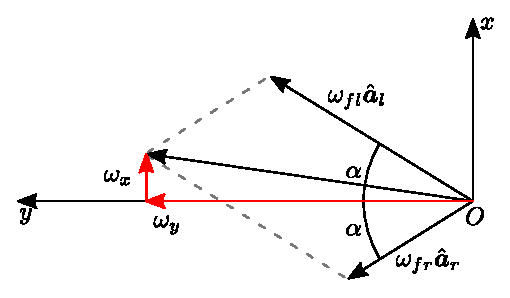
\includegraphics[width=.8\linewidth]{figures/sum_diff_mod.eps}
	\caption{\small Having incident rotation axes, the \gls{ocs} allows to control both the robot roll and pitch. Notice that the roll is influenced by the difference of the angular speeds of the flywheels, $\omega_x = \left(\omega_{fl} - \omega_{fr}\right)\sin(\alpha)$. On the contrary, the pitch depends on the sum of the angular speeds $\omega_y = \left(\omega_{fl} -  \omega_{fr}\right)\cos(\alpha)$.}
	\label{fig:sum-diff}
\end{figure}

\subsection{Inertia Selection}
Once the desired inertia $I_f$ is chosen, according to the 2-D Elroy's Beanie model, it is used to realize the 3-D \gls{ocs} (Fig. \ref{fig:flywheel}). 
\begin{figure}
	\centering
	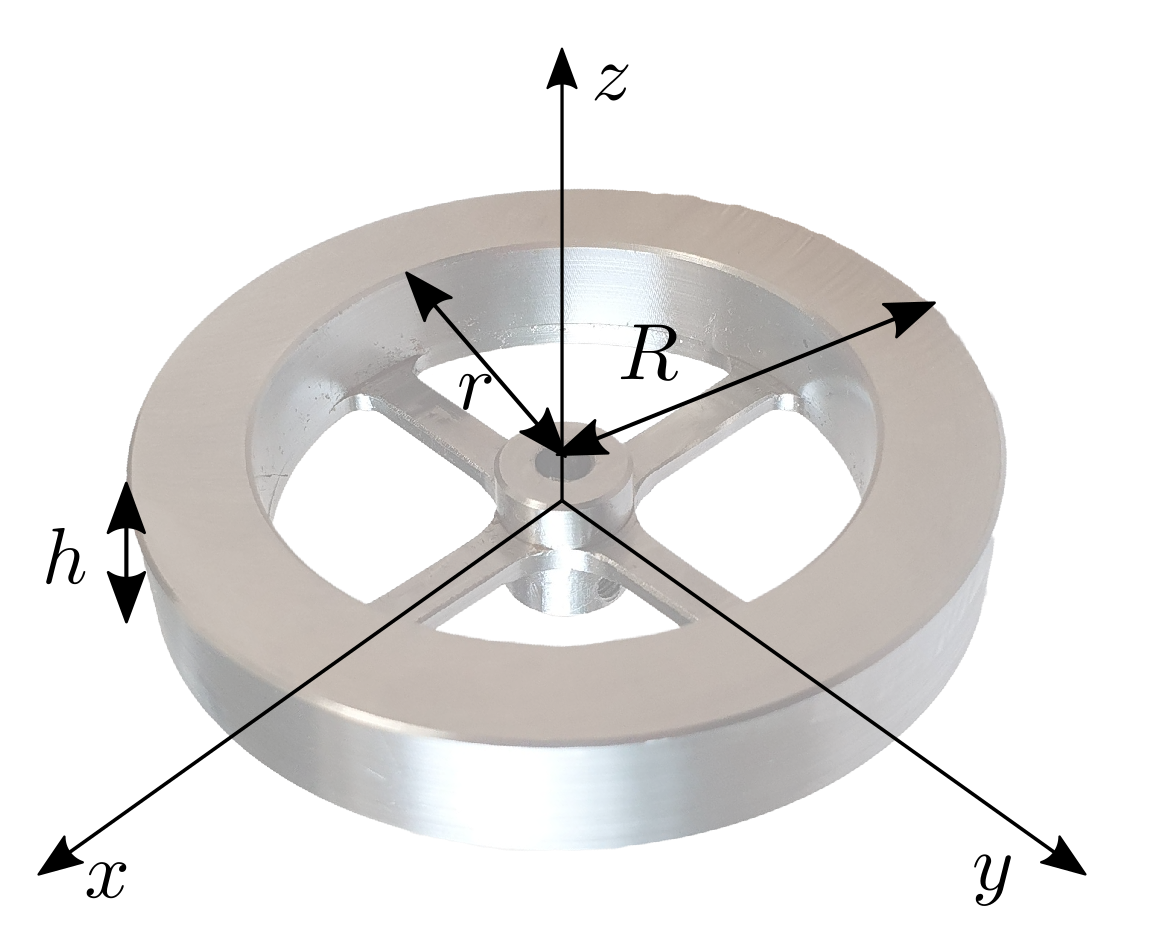
\includegraphics[width=0.7\linewidth]{figures/flywheel_opaque.png}
	\caption{\small The final design of the flywheel, shown together with its inertia principal axes. Here, $h$ is the wheel thickness, $r$ is the inner radius of the wheel and $R$ is the outer one.}
	\label{fig:flywheel}
\end{figure}
We decided to design the flywheels in the shape of hollow cylinders. This shape increases the inertia by locating the mass far away from the rotation axis. The inertia tensor expressed in its principal axes, $\bm{I}_f = \mathrm{diag}\left\{ I_{f, xx}, \, I_{f, yy}, \, I_{f, zz}  \right\}$, depends on the cylinders inner and outer radii, $r$ and $R$, its height $h$ and the material density $\rho$:
\begin{equation}
\begin{split}
I_{f, xx} = I_{f, yy} &= \frac{1}{12}\pi \rho h \left(3\left(R^4 - r^4\right) + h^2\left(R^2 - r^2\right)\right) \\
I_{f, zz} &= \frac{1}{2}\pi \rho h \left(R^4 - r^4\right)
\end{split}
\end{equation}
Notice that in the Elroy's Beanie model, there is a single body that models the complete \gls{ocs}. The inertia introduced in the Elroy's Beanie model has to be split between the two flywheels: $I_{f, zz} = I_f/\left(2\cos(\alpha)\right)$. 
The parameters $R$ and $h$ can be set to have a compact \gls{ocs} and $\rho$ depends on the chosen material, that is stainless steel in our case. The inner radius $r$ can be adjusted to obtain the desired inertia. Spokes with negligible mass connect the wheel to the motor shaft. All the parameters are reported in Table \ref{tab:dim_fw}, together with the selected inertia and mass of a single flywheel.
\begin{table}
	\centering
	\caption{\small Size and dynamic parameters of a single flywheel}
	\begin{tabular}{ccc}
		Parameter & Value & Unit \\
		\hline
		\hline
		$r$ & $2.20\cdot 10^{-2}$ & $\mathrm{m}$ \\
		$R$ & $3.00\cdot 10^{-2}$ & $\mathrm{m}$ \\
		$h$   & $1.02\cdot 10^{-2}$ & $\mathrm{m}$ \\
		$\rho$   & $7.860 \cdot 10^{3}$ & $\mathrm{kg/m^3}$ \\
		$m$   & $1.02\cdot 10^{-1}$ & $\mathrm{kg}$ \\
		$I_{xx}, I_{yy}$   & $3.64 \cdot 10^{-5}$ & $\mathrm{kg \cdot m^2}$ \\
		$I_{zz}$   & $7.11 \cdot 10^{-5}$ & $ \mathrm{kg \cdot m^2}$ \\
	\end{tabular}
	\label{tab:dim_fw}
\end{table}

\subsection{Flywheels Control Law}
\label{subsec:control_law}
To derive a control law based on the robot base orientation, we make use of \eqref{eq:cons_ang_mom}, expressing all the contributions to the time derivative of total angular momentum with the respect to the base reference frame:
\begin{equation*}
\tensor[_b]{\bm{I}}{_f} \, \tensor[_b]{\dot{\bm{\omega}}}{_f} + \tensor[_b]{\bm{I}}{_r} \tensor[_b]{\dot{\bm{\omega}}}{_r} + \tensor[_b]{\bm{\omega}}{_r} \times \left( \tensor[_b]{\bm{I}}{_r} \tensor[_b]{\bm{\omega}}{_r}\right) = 0
\end{equation*}
From this expression, we can define the moment on the base caused by the acceleration of the flywheels, that can be used as a feedback torque $\bm{\tau}_{fb}$:
\begin{equation*}
\begin{split}
\bm{\tau}_{fb} &= \bm{I}_f \dot{\bm{\omega}}_f \\
&= - \tensor[_b]{\bm{I}}{_r} \dot{\bm{\omega}}_b - \tensor[_b]{\bm{\omega}}{_r} \times \left( \tensor[_b]{\bm{I}}{_r} \tensor[_b]{\bm{\omega}}{_r}\right)
\end{split}
\end{equation*}
We can use the PD action $\bm{K}_p \bm{e} + \bm{K}_d \dot{\bm{e}_r}$, where $\bm{K}_p$ and $\bm{K}_d$ are diagonal and positive-definite gain matrices for the error in attitude and angular velocity.
The orientation error $\bm{e} \in SO(3)$ needs the algebra of the special rotational group to be computed. To avoid singular configurations, we represent the orientation with quaternions.
The derivative error can be computed using $\dot{\bm{e}} = \tensor[_b]{\bm{\omega}}{_r^{des}} - \tensor[_b]{\bm{\omega}}{_r}$, in which $\tensor[_b]{\bm{\omega}}{_r^{des}}$ and $\tensor[_b]{\bm{\omega}}{_r}$ are, respectively, the desired and actual angular velocity of the base:
\begin{equation*}
\bm{\tau}_{fb} = - \tensor[_b]{\bm{I}}{_r} \left(\bm{K}_p \bm{e} + \bm{K}_d \dot{\bm{e}}\right) - \tensor[_b]{\bm{\omega}}{_r} \times \left( \tensor[_b]{\bm{I}}{_r} \tensor[_b]{\bm{\omega}}{_r}\right)
\end{equation*}
Projecting the moment $\bm{\tau}_{fb}$ onto the flywheel axes with $\bm{C}^T$, we obtain the control action $\bm{u}$
\begin{equation}
\label{eq:ctrl_law}
\bm{u} = \bm{C}^T \bm{\tau}_{fb}
\end{equation}

\section{Results of Simulations}
\label{sec:simulations}
To validate our \gls{ocs}, we present three simulations on different scenarios. We want to test the capability of the proposed approach to: 
reject a disturbance when the robot is in the flight phase of a jump, damp trunk oscillations after the touch-down, 
and work in parallel with the joints of the legs to achieve a highly dynamic motion. 
All the simulations are performed in Gazebo. The robot full dynamics is modeled with Pinocchio \cite{carpentier2019pinocchio}. The references for the joints of the legs are computed off-line using Crocoddyl \cite{mastalli2020crocoddyl} and tracked with a PD joint controller. The \gls{ocs} is commanded to 
track base orientation references using the control law introduced in Subsection \ref{subsec:control_law}.\footnote{The video with all the simulations is available at web link \url{https://www.dropbox.com/scl/fo/wevvl0zvfp8gofie6x7rw/h?dl=0&rlkey=pap76cr813a0skrvrxl7qgrb9}.}

%this is the main test! 
The necessity of having an \gls{ocs} is revealed with the first test: disturbance that occurs when the robot has no contact with the ground. 
During the flight phase of a forward jump, $0.1~\mathrm{s}$ after the lift-off, an external disturbance moment is applied to the robot base, deflecting the robot orientation: this disturbance is set to $\bm{\tau}_{dist} = \left[\begin{array}{ccc}
0.2 & 0.8 & 0.0
\end{array}
\right]^T \ \mathrm{N \cdot m}$ and applied for $0.05 \ \mathrm{s}$. 
If the flywheels are not used, Solo12 falls after the touch-down. Instead, 
using the flywheels %pairing the legs joint PD controller with \ref{eq:ctrl_law},
it is possible to drive the robot to a safe configuration after the landing (Fig. \ref{fig:fw_jump}), without need to implement of a specific landing strategy, as the one in \cite{jeon2021real}.
\begin{figure}
	\centering
	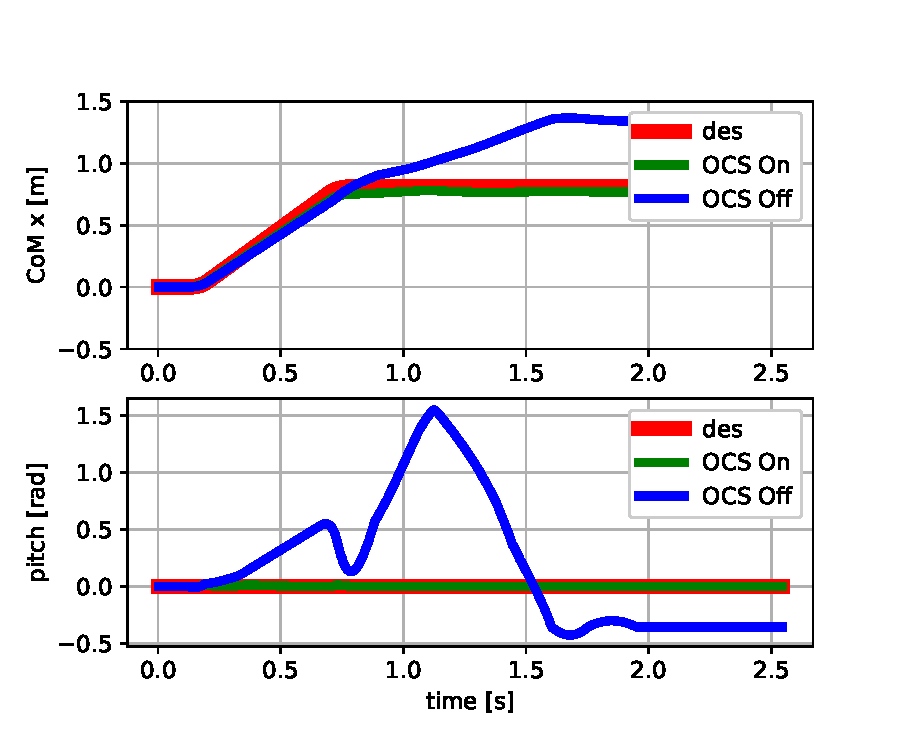
\includegraphics[width=1\linewidth]{figures/fw_jump.eps}
	\caption{\small First Test: simulation results showing the $\mathrm{CoM}_x$ and pitch trajectory vs. time plots. A disturbance moment $\bm{\tau}_{dist}$ on the trunk can be compensated only if the \gls{ocs} is enabled. If it is disabled, the robot is unable to restore a safe configuration after the touch-down and eventually falls.}
	\label{fig:fw_jump}
\end{figure}

In the second test, we demonstrate the ability of the \gls{ocs} to reorient the base.
We let the robot fall from a height of $1 \ \mathrm{m}$ with an initial pitch orientation of $30^\circ$ and zero base angular velocity.
If we do not actuate the flywheels, the robot touches the ground with the same initial orientation and the trunk oscillates. If the \gls{ocs}is enabled, it drives the robot base to be horizontal when it is still in the air and the oscillations after the touch-down are drastically reduced, both in the pitch angle and forward direction (Fig. \ref{fig:fall_plot}).
\begin{figure}
	\centering
	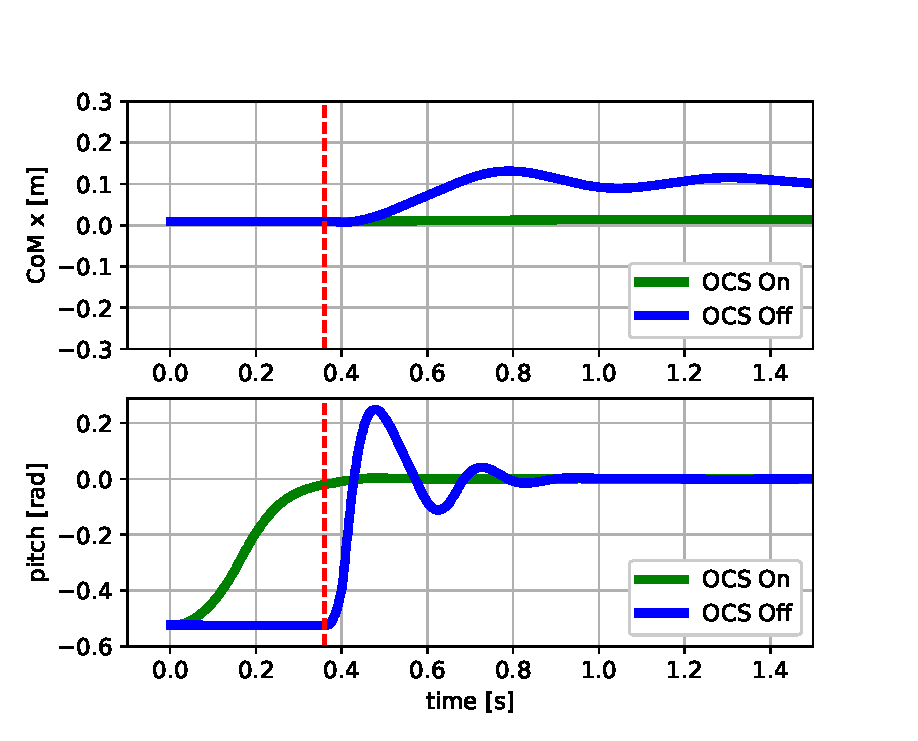
\includegraphics[width=1\linewidth]{figures/fall_plot.eps}
	\caption{\small Second Test: simulation results showing the $\mathrm{CoM}_x$ and pitch trajectory vs. time plots. The \gls{ocs} drives the robot orientation during a fall to be horizontal. This allows to damp for damping the base oscillations after the touch-down (vertical dashed line), even without implementing a landing strategy}
	\label{fig:fall_plot}
\end{figure}


%In a second test, we demonstrate the versatility use the presented \gls{ocs} to dump the base oscillations generated at the landing. 
%% , even though we designed it to control the orientation during the flight phase.
%To demonstrate this feature, we use the same joint trajectory to perform two simulations: 
%in the first, we control the flywheels to track an orientation parallel to the ground, while in the other they are not actuated.
%The joint trajectory realizes a jump with a height of $0.4 \ \mathrm{m}$, a forward distance of $0.8 \ \mathrm{m}$, and a flight phase of $0.5 \ \mathrm{s}$. \MF{why you detail here the jump and not before? is the same jump?}
%The results point out the possibility to use this device even when the angular momentum is not conserved (i.e. when contacts are present).



Finally, we demonstrate how flywheels can alleviate the effort of the leg joints to achieve a highly dynamic motion: a back-flip. 
For this, we target a space application carrying out a simulation with Moon gravity ($1.62 \ \mathrm{m/s^2}$).
In this way, it is possible to obtain high jumps with a long flight phase, without having to select more powerful actuators.  
The leg joint trajectory computed off-line describes a purely vertical jump of $1 \ \mathrm{m}$, having a flight phase that lasts $2 \ \mathrm{s}$.
Right after the lift-off, the flywheels start the reorientation task of performing a back-flip, that is a spin of $360^\circ$ on the pitch.
For this maneuver, the value of the incident angle $\alpha$ is set to $0^\circ$ since no roll rotation is required.
% and it is preferred to use all the contributions of the \gls{ocs} on the pitch.
Our hardware design allows the manual change of this value before performing the task.
This simulation demonstrates that the \gls{ocs} alleviate the effort to be applied on the legs: indeed, that it would not have been possible to do a back-flip without the flywheels because the legs are used only to achieve the linear motion.


\section{Conclusions}
\label{sec:conclusions}

In this work, we have presented the design of a novel \gls{ocs}, composed of two flywheels, that enables to control the trunk of a legged robot platform, 
increasing the accuracy of aerial maneuvers during the under-actuated phases (i.e., flight phase) as well as 
enhancing stability when in contact by damping oscillations.
The novelty of the design, that involves the flywheels to be attached with incident rotational axes on the trunk, allows to control the orientation
in both the roll and pitch directions while keeping the device compact. Their effect is optimized considering the inertial property of the mechanical structure. 
Several simulations are reported with the quadruped Solo12 that demonstrate the effectiveness of the proposed approach to: 
reject disturbances during the flight phase, stabilize the platform after the touch-down even in absence of a specific landing strategy and 
achieve a fast reorientation maneuver (a back-flip) in a reduced gravity environment. 

In future works, we plan to demonstrate our concept performing experiment with the real platform. The control strategy for defining the base desired angular velocity can be improved using \gls{nmpc}, that takes into consideration the future samples of the orientation reference.
We expect this feature will allows the stabilization of the yaw to a desired value, that if it is not locally controllable, enhancing the non-holonomy property of the angular momentum, i.e. doing a preliminary roll and pitch maneuver. 
A control strategy that may lead to the same result is dynamic feedback linearization, widely used for flight with quadricopters.



\small
\section*{Acknowledgements}	
All the authors want to thank Dr. Roy Featherstone for interesting tips that started this work. 
\newline
The publication was created with the co-financing of the European Union FSE-REACT-EU, PON Research and Innovation 2014-2020 DM1062 / 2021.





\printbibliography
\end{document}